\documentclass[10pt,ignorenonframetext,,aspectratio=149]{beamer}
\usefonttheme{serif} % use mainfont rather than sansfont for slide text
\setbeamertemplate{caption}[numbered]
\setbeamertemplate{caption label separator}{: }
\setbeamercolor{caption name}{fg=normal text.fg}
\usepackage{lmodern}
\usepackage{amssymb,amsmath}
\usepackage{ifxetex,ifluatex}
\usepackage{fixltx2e} % provides \textsubscript
\ifnum 0\ifxetex 1\fi\ifluatex 1\fi=0 % if pdftex
  \usepackage[T1]{fontenc}
  \usepackage[utf8]{inputenc}
\else % if luatex or xelatex
  \ifxetex
    \usepackage{mathspec}
  \else
    \usepackage{fontspec}
  \fi
  \defaultfontfeatures{Ligatures=TeX,Scale=MatchLowercase}
  \newcommand{\euro}{€}
    \setmainfont[]{Open Sans}
\fi
% use upquote if available, for straight quotes in verbatim environments
\IfFileExists{upquote.sty}{\usepackage{upquote}}{}
% use microtype if available
\IfFileExists{microtype.sty}{%
\usepackage{microtype}
\UseMicrotypeSet[protrusion]{basicmath} % disable protrusion for tt fonts
}{}
\usepackage{color}
\usepackage{fancyvrb}
\newcommand{\VerbBar}{|}
\newcommand{\VERB}{\Verb[commandchars=\\\{\}]}
\DefineVerbatimEnvironment{Highlighting}{Verbatim}{commandchars=\\\{\}}
% Add ',fontsize=\small' for more characters per line
\usepackage{framed}
\definecolor{shadecolor}{RGB}{248,248,248}
\newenvironment{Shaded}{\begin{snugshade}}{\end{snugshade}}
\newcommand{\AlertTok}[1]{\textcolor[rgb]{0.94,0.16,0.16}{#1}}
\newcommand{\AnnotationTok}[1]{\textcolor[rgb]{0.56,0.35,0.01}{\textbf{\textit{#1}}}}
\newcommand{\AttributeTok}[1]{\textcolor[rgb]{0.77,0.63,0.00}{#1}}
\newcommand{\BaseNTok}[1]{\textcolor[rgb]{0.00,0.00,0.81}{#1}}
\newcommand{\BuiltInTok}[1]{#1}
\newcommand{\CharTok}[1]{\textcolor[rgb]{0.31,0.60,0.02}{#1}}
\newcommand{\CommentTok}[1]{\textcolor[rgb]{0.56,0.35,0.01}{\textit{#1}}}
\newcommand{\CommentVarTok}[1]{\textcolor[rgb]{0.56,0.35,0.01}{\textbf{\textit{#1}}}}
\newcommand{\ConstantTok}[1]{\textcolor[rgb]{0.00,0.00,0.00}{#1}}
\newcommand{\ControlFlowTok}[1]{\textcolor[rgb]{0.13,0.29,0.53}{\textbf{#1}}}
\newcommand{\DataTypeTok}[1]{\textcolor[rgb]{0.13,0.29,0.53}{#1}}
\newcommand{\DecValTok}[1]{\textcolor[rgb]{0.00,0.00,0.81}{#1}}
\newcommand{\DocumentationTok}[1]{\textcolor[rgb]{0.56,0.35,0.01}{\textbf{\textit{#1}}}}
\newcommand{\ErrorTok}[1]{\textcolor[rgb]{0.64,0.00,0.00}{\textbf{#1}}}
\newcommand{\ExtensionTok}[1]{#1}
\newcommand{\FloatTok}[1]{\textcolor[rgb]{0.00,0.00,0.81}{#1}}
\newcommand{\FunctionTok}[1]{\textcolor[rgb]{0.00,0.00,0.00}{#1}}
\newcommand{\ImportTok}[1]{#1}
\newcommand{\InformationTok}[1]{\textcolor[rgb]{0.56,0.35,0.01}{\textbf{\textit{#1}}}}
\newcommand{\KeywordTok}[1]{\textcolor[rgb]{0.13,0.29,0.53}{\textbf{#1}}}
\newcommand{\NormalTok}[1]{#1}
\newcommand{\OperatorTok}[1]{\textcolor[rgb]{0.81,0.36,0.00}{\textbf{#1}}}
\newcommand{\OtherTok}[1]{\textcolor[rgb]{0.56,0.35,0.01}{#1}}
\newcommand{\PreprocessorTok}[1]{\textcolor[rgb]{0.56,0.35,0.01}{\textit{#1}}}
\newcommand{\RegionMarkerTok}[1]{#1}
\newcommand{\SpecialCharTok}[1]{\textcolor[rgb]{0.00,0.00,0.00}{#1}}
\newcommand{\SpecialStringTok}[1]{\textcolor[rgb]{0.31,0.60,0.02}{#1}}
\newcommand{\StringTok}[1]{\textcolor[rgb]{0.31,0.60,0.02}{#1}}
\newcommand{\VariableTok}[1]{\textcolor[rgb]{0.00,0.00,0.00}{#1}}
\newcommand{\VerbatimStringTok}[1]{\textcolor[rgb]{0.31,0.60,0.02}{#1}}
\newcommand{\WarningTok}[1]{\textcolor[rgb]{0.56,0.35,0.01}{\textbf{\textit{#1}}}}
\usepackage{longtable,booktabs}
\usepackage{caption}
% These lines are needed to make table captions work with longtable:
\makeatletter
\def\fnum@table{\tablename~\thetable}
\makeatother
\usepackage{graphicx,grffile}
\makeatletter
\def\maxwidth{\ifdim\Gin@nat@width>\linewidth\linewidth\else\Gin@nat@width\fi}
\def\maxheight{\ifdim\Gin@nat@height>\textheight0.8\textheight\else\Gin@nat@height\fi}
\makeatother
% Scale images if necessary, so that they will not overflow the page
% margins by default, and it is still possible to overwrite the defaults
% using explicit options in \includegraphics[width, height, ...]{}
\setkeys{Gin}{width=\maxwidth,height=\maxheight,keepaspectratio}

% Comment these out if you don't want a slide with just the
% part/section/subsection/subsubsection title:
\AtBeginPart{
  \let\insertpartnumber\relax
  \let\partname\relax
  \frame{\partpage}
}
\AtBeginSection{
  \let\insertsectionnumber\relax
  \let\sectionname\relax
  \frame{\sectionpage}
}
\AtBeginSubsection{
  \let\insertsubsectionnumber\relax
  \let\subsectionname\relax
  \frame{\subsectionpage}
}

\setlength{\emergencystretch}{3em}  % prevent overfull lines
\providecommand{\tightlist}{%
  \setlength{\itemsep}{0pt}\setlength{\parskip}{0pt}}
\setcounter{secnumdepth}{0}

\title{Pre-processing data Teks menggunakan R}
\subtitle{(Pelatihan data sains menggunakan R dan Gephi)}
\author{Ujang Fahmi}
\date{}

%% Here's everything I added.
%%--------------------------

\usepackage{graphicx}
\usepackage{rotating}
%\setbeamertemplate{caption}[numbered]
\usepackage{hyperref}
\usepackage{caption}
\usepackage[normalem]{ulem}
%\mode<presentation>
\usepackage{wasysym}
%\usepackage{amsmath}


% Get rid of navigation symbols.
%-------------------------------
\setbeamertemplate{navigation symbols}{}

% Optional institute tags and titlegraphic.
% Do feel free to change the titlegraphic if you don't want it as a Markdown field.
%----------------------------------------------------------------------------------
\institute{Pelajaran ke-3}

% \titlegraphic{\includegraphics[width=0.3\paperwidth]{\string~/Dropbox/teaching/clemson-academic.png}} % <-- if you want to know what this looks like without it as a Markdown field. 
% -----------------------------------------------------------------------------------------------------
\titlegraphic{
\includegraphics[width=0.3\paperwidth]{styles/sadasa.png}}

% Some additional title page adjustments.
%----------------------------------------
\setbeamertemplate{title page}[empty]
%\date{}
\setbeamerfont{subtitle}{size=\small}

\setbeamercovered{transparent}

% Some optional colors. Change or add as you see fit.
%---------------------------------------------------
\definecolor{clemsonpurple}{HTML}{522D80}
 \definecolor{clemsonorange}{HTML}{F66733}
\definecolor{uiucblue}{HTML}{003C7D}
\definecolor{uiucorange}{HTML}{F47F24}


% Some optional color adjustments to Beamer. Change as you see fit.
%------------------------------------------------------------------
\setbeamercolor{frametitle}{fg=clemsonpurple,bg=white}
\setbeamercolor{title}{fg=clemsonpurple,bg=white}
\setbeamercolor{local structure}{fg=clemsonpurple}
\setbeamercolor{section in toc}{fg=clemsonpurple,bg=white}
% \setbeamercolor{subsection in toc}{fg=clemsonorange,bg=white}
\setbeamercolor{footline}{fg=clemsonpurple!50, bg=white}
\setbeamercolor{block title}{fg=clemsonorange,bg=white}


\let\Tiny=\tiny


% Sections and subsections should not get their own damn slide.
%--------------------------------------------------------------
\AtBeginPart{}
\AtBeginSection{}
\AtBeginSubsection{}
\AtBeginSubsubsection{}

% Suppress some of Markdown's weird default vertical spacing.
%------------------------------------------------------------
\setlength{\emergencystretch}{0em}  % prevent overfull lines
\setlength{\parskip}{0pt}

% Allow for those simple two-tone footlines I like. 
% Edit the colors as you see fit.
%--------------------------------------------------
\defbeamertemplate*{footline}{my footline}{%
    \ifnum\insertpagenumber=1
    \hbox{%
        \begin{beamercolorbox}[wd=\paperwidth,ht=.8ex,dp=1ex,center]{}%
      % empty environment to raise height
        \end{beamercolorbox}%
    }%
    \vskip0pt%
    \else%
        \Tiny{%
            \hfill%
		\vspace*{1pt}%
            \insertframenumber/\inserttotalframenumber \hspace*{0.1cm}%
            \newline%
            \color{clemsonpurple}{\rule{\paperwidth}{0.4mm}}\newline%
            \color{clemsonorange}{\rule{\paperwidth}{.4mm}}%
        }%
    \fi%
}

% Various cosmetic things, though I must confess I forget what exactly these do and why I included them.
%-------------------------------------------------------------------------------------------------------
\setbeamercolor{structure}{fg=blue}
\setbeamercolor{local structure}{parent=structure}
\setbeamercolor{item projected}{parent=item,use=item,fg=clemsonpurple,bg=white}
\setbeamercolor{enumerate item}{parent=item}

% Adjust some item elements. More cosmetic things.
%-------------------------------------------------
\setbeamertemplate{itemize item}{\color{clemsonpurple}$\bullet$}
\setbeamertemplate{itemize subitem}{\color{clemsonpurple}\scriptsize{$\bullet$}}
\setbeamertemplate{itemize/enumerate body end}{\vspace{.6\baselineskip}} % So I'm less inclined to use \medskip and \bigskip in Markdown.

% Automatically center images
% ---------------------------
% Note: this is for ![](image.png) images
% Use "fig.align = "center" for R chunks

\usepackage{etoolbox}

\AtBeginDocument{%
  \letcs\oig{@orig\string\includegraphics}%
  \renewcommand<>\includegraphics[2][]{%
    \only#3{%
      {\centering\oig[{#1}]{#2}\par}%
    }%
  }%
}

% I think I've moved to xelatex now. Here's some stuff for that.
% --------------------------------------------------------------
% I could customize/generalize this more but the truth is it works for my circumstances.

\ifxetex
\setbeamerfont{title}{family=\fontspec{Titillium Web}}
\setbeamerfont{frametitle}{family=\fontspec{Titillium Web}}
\usepackage[font=small,skip=0pt]{caption}
 \else
 \fi

% Okay, and begin the actual document...

\begin{document}
\frame{\titlepage}

\begin{frame}
Salam kenal dan selamat datang.

Semoga kita semua bisa saling berbagi pengalaman dan pengetahuan. Saya
adalah Ujang Fahmi, Co-founder dan mentor Sadasa Academy.

\vspace{0.1in}

Jika anda berada dan sedang membaca tutorial ini, maka kemungkinan anda
adalah orang yang sedang ingin belajar data sains, atau mungkin
ditugaskan untuk mempelajari R oleh institusi atau organisasi anda. Sama
seperti saya dulu, dimana tanpa latar belakang enginering saya
didiharuskan untuk belajar R, demi menyelesaikan tugas akhir dan
akhirnya jadilah seperti saya sekarang ini.

\vspace{0.1in}

Satu hal yang pasti, ini adalah langkah pertama dari banyak langkah yang
harus dilalui, entah melalui lembaga resmi atau belajar secara mandiri.
Jadi selamat belajar!!!

\vspace{0.1in}

Ujang Fahmi,

Yogyakarta, 2021-09-17
\end{frame}

\hypertarget{text-mining}{%
\section{Text Mining?}\label{text-mining}}

\begin{frame}{Text Mining?}
Text mining juga merujuk pada text data mining mirip dengan teks
analitik, yaitu sebuah proses mendapatkan informasi yang berkualitas
dari teks. Hal ini melibatkan penggunaan komputer untuk observasi, dan
\textbf{informasi yang sebelumnya belum diketahui}.

Text mining melibatkan teknik dan metode interdisiplin seperti
pemerograman komputer untuk memproses data tidak terstruktur dalam
jumlah besar dan linguistik untuk memahami dan mengambil intiusi tentang
penggunaan bahasa.

source:
\href{https://www.tex-ai.com/5-important-text-mining-techniques-in-use-today/}{text.ai}
\end{frame}

\hypertarget{metode-analisis}{%
\subsection{Metode analisis}\label{metode-analisis}}

\begin{frame}{Metode analisis}
\begin{columns}[T]
\begin{column}{0.5\textwidth}
\begin{enumerate}
\tightlist
\item
  Term-based Method (Each term is associated with a value, known as
  weight)
\item
  Phrase-based Method (This method analyses a document based on phrases
  which carry more information than a single term)
\item
  Concept-based Method (This model tries to analyses a term on a
  document or sentence level by finding a significant matching term)
\item
  Pattern Taxonomy Method (Relation between terms to form taxonomy,
  which is a tree-like structure)
\item
  Metode hibrida pengolahan teks (e.g CADS)
\end{enumerate}
\end{column}

\begin{column}{0.5\textwidth}
\begin{figure}
\centering
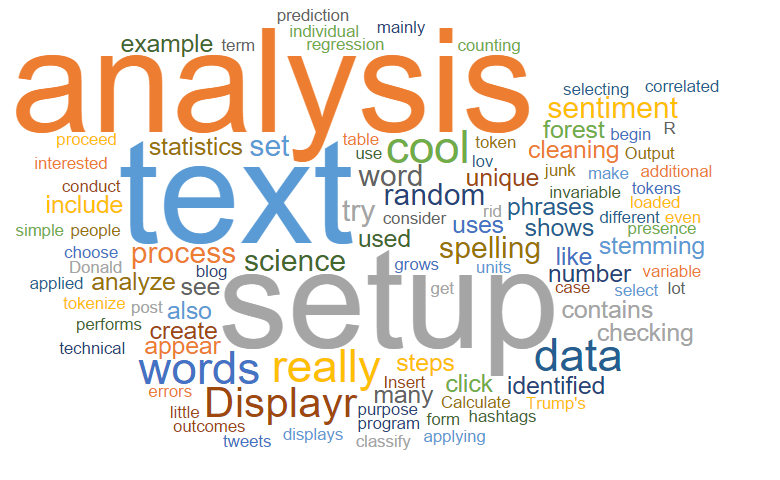
\includegraphics{images/img1.png}
\caption{Buzz words}
\end{figure}
\end{column}
\end{columns}
\end{frame}

\hypertarget{teknik-analisis}{%
\subsection{Teknik analisis}\label{teknik-analisis}}

\begin{frame}[fragile]{Teknik analisis}
\begin{enumerate}
\item
  \textbf{Extraction of Information} (The information extraction
  technique focuses a lot on identifying the extraction of attributes,
  entities, along with their relationship with unstructured or
  semi-structured texts)
\item
  \textbf{Retrieval of Information} (This technique makes use of
  information retrieval systems that make use of various algorithms that
  track and monitor user behaviour and also determine related data
  accordingly)
\item
  \textbf{Categorization} (This is a text mining technique which is a
  \texttt{supervised} learning form where the usual language texts are
  set to a pre-defined bunch of topics depending on their content)
\item
  \textbf{Clustering} (Clustering helps identify structures that are
  intrinsic in nature within text information and organize them in
  clusters or relevant subgroups for further analysis)
\item
  \textbf{Summarization} (Text summarization allows you to browse
  through various text sources in order to create summaries of texts
  which contain large amounts of information that are insightful in a
  concise format)
\end{enumerate}
\end{frame}

\hypertarget{proses-analisis}{%
\subsection{Proses Analisis}\label{proses-analisis}}

\begin{frame}{Proses Analisis}
\begin{columns}[T]
\begin{column}{0.5\textwidth}
\begin{enumerate}
\tightlist
\item
  Mendapatkan data (umumnya tidak/belum terstruktur)
\item
  Melakukan pre-proccessing (melibatkan data wrangling dan cleansing)
\item
  Membuat data terstruktur
\item
  Menyimpan dan menganalisis
\end{enumerate}
\end{column}

\begin{column}{0.5\textwidth}
\begin{figure}
\centering
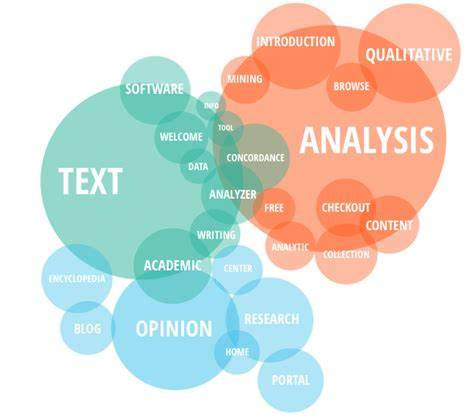
\includegraphics{images/img2.jpeg}
\caption{Buzz words}
\end{figure}
\end{column}
\end{columns}
\end{frame}

\hypertarget{memanfaatkan-regex-regular-expression}{%
\section{Memanfaatkan Regex (Regular
Expression)}\label{memanfaatkan-regex-regular-expression}}

\begin{frame}{Memanfaatkan Regex (Regular Expression)}
A regular expression (shortened as regex or regexp; also referred to as
rational expression) is a sequence of characters that specifies a search
pattern. Usually such patterns are used by string-searching algorithms
for ``find'' or ``find and replace'' operations on strings, or for input
validation. It is a technique developed in theoretical computer science
and formal language theory.
\href{https://en.wikipedia.org/wiki/Regular_expression}{wikipedia}
\end{frame}

\hypertarget{penggunaan-regex}{%
\subsection{Penggunaan regex}\label{penggunaan-regex}}

\begin{frame}{Penggunaan regex}
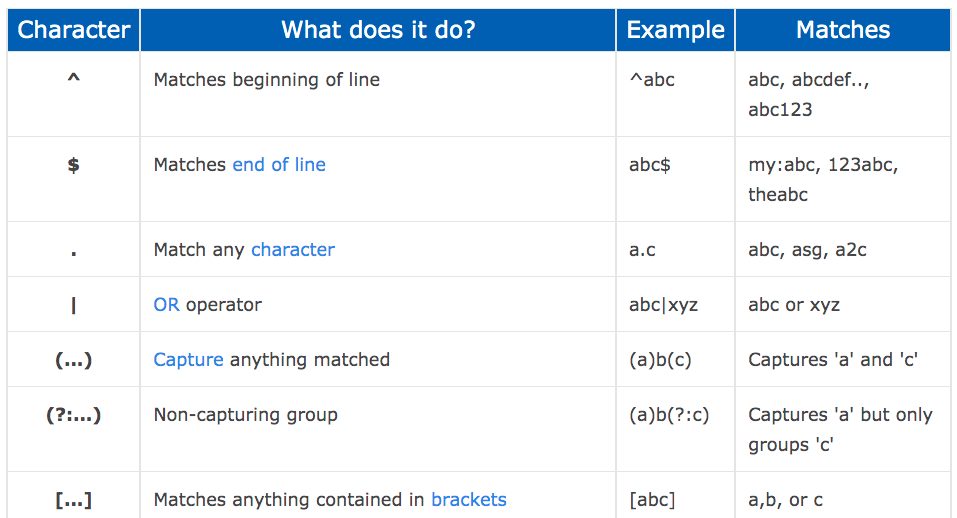
\includegraphics{images/img3.png} source:
\href{https://www.computerhope.com/jargon/r/regex.htm}{computerhope}
\end{frame}

\hypertarget{pra-pemerosesan-data-teks}{%
\section{Pra-pemerosesan data teks}\label{pra-pemerosesan-data-teks}}

\begin{frame}{Pra-pemerosesan data teks}
Data teks yang umumnya tidak terstruktur biasanya juga masih banyak
elemen yang tidak diperlukan dalam analisis. Oleh karena itu biasanya
kita perlu membersihkan noise nya terlebih dahulu.
\end{frame}

\hypertarget{noise-removal}{%
\subsection{Noise removal}\label{noise-removal}}

\begin{frame}{Noise removal}
Noise removal disini termasuk tanda html (html tags, spasi yang lebih,
tanda baca dan sambung, serta menyergamkan teks)
\end{frame}

\begin{frame}[fragile]{Remove HTML tags}
\protect\hypertarget{remove-html-tags}{}
html tags yang umum ada dalam teks adalah url. Urls biasanya diawali
dengan kelompok karakter spesifik, seperti:

\begin{itemize}
\tightlist
\item
  http
\item
  https
\item
  www
\item
  etc
\end{itemize}

\href{https://www.gastonsanchez.com/r4strings/}{Buku untuk belajar regex
di R/Handling Strings With R}

\begin{Shaded}
\begin{Highlighting}[]
\NormalTok{teks }\OtherTok{=} \StringTok{"Bpbd... }
\StringTok{        https://instagram.com/p/CT5xmXMP\_xq/?utm\_medium=twitter, }
\StringTok{        www.dodoremi.com, }
\StringTok{        pic.twitter..."}
\CommentTok{\# teks}

\FunctionTok{library}\NormalTok{(stringr)}
\NormalTok{teks }\OtherTok{=} \FunctionTok{gsub}\NormalTok{(}\StringTok{" ?(f|ht)(tp)(s?)(://)(.*)[.|/](.*)"}\NormalTok{, }\StringTok{""}\NormalTok{, teks)}
\end{Highlighting}
\end{Shaded}
\end{frame}

\begin{frame}[fragile]{Remove extra whitespaces}
\protect\hypertarget{remove-extra-whitespaces}{}
\begin{Shaded}
\begin{Highlighting}[]
\NormalTok{teks }\OtherTok{=} \StringTok{" jagalah 3m, Menjaga Jarak, }
\StringTok{         kebersihan, dan menjaga hatii......."}
\NormalTok{teks}

\FunctionTok{library}\NormalTok{(textclean)}

\CommentTok{\# extra sapce}
\FunctionTok{replace\_white}\NormalTok{(teks)}

\CommentTok{\# white space di depan/belakang}
\FunctionTok{str\_trim}\NormalTok{(}\AttributeTok{string =}\NormalTok{ teks, }\AttributeTok{side =} \StringTok{"both"}\NormalTok{)}
\end{Highlighting}
\end{Shaded}
\end{frame}

\begin{frame}[fragile]{Remove special characters}
\protect\hypertarget{remove-special-characters}{}
\begin{Shaded}
\begin{Highlighting}[]
\NormalTok{teks }\OtherTok{=} \StringTok{" jagalah 3m, Menjaga jarak, }
\StringTok{         kebersihan, dan menjaga hatii......."}

\FunctionTok{library}\NormalTok{(textclean)}
\NormalTok{teks }\OtherTok{=} \FunctionTok{replace\_non\_ascii}\NormalTok{(teks)}
\NormalTok{teks}
\end{Highlighting}
\end{Shaded}
\end{frame}

\begin{frame}[fragile]{Remove Punctuations}
\protect\hypertarget{remove-punctuations}{}
\begin{Shaded}
\begin{Highlighting}[]
\NormalTok{teks }\OtherTok{=} \StringTok{" jagalah 3m, menjaga jarak, }
\StringTok{         kebersihan, dan menjaga hatii......."}

\NormalTok{teks }\OtherTok{=} \FunctionTok{gsub}\NormalTok{(}\AttributeTok{pattern =} \StringTok{"[[:punct:]]"}\NormalTok{, }\AttributeTok{replacement =} \StringTok{""}\NormalTok{, teks)}
\NormalTok{teks}
\end{Highlighting}
\end{Shaded}
\end{frame}

\hypertarget{lower-atau-upper-case}{%
\subsection{Lower atau Upper Case}\label{lower-atau-upper-case}}

\begin{frame}[fragile]{Lower atau Upper Case}
\begin{Shaded}
\begin{Highlighting}[]
\NormalTok{teks }\OtherTok{=} \StringTok{"jagalah 3m, menjaga jarak"}

\NormalTok{teks }\OtherTok{=} \FunctionTok{toupper}\NormalTok{(teks)}
\NormalTok{teks}
\NormalTok{teks }\OtherTok{=} \FunctionTok{tolower}\NormalTok{(teks)}
\NormalTok{teks}
\end{Highlighting}
\end{Shaded}
\end{frame}

\hypertarget{pembersihan-kata-sambung}{%
\subsection{Pembersihan kata sambung}\label{pembersihan-kata-sambung}}

\begin{frame}[fragile]{Pembersihan kata sambung}
Untuk membersihkan kata sambung kita membutuhkan kamus kata sambung.
Kamus ini biasanya sudah dibuat terlebih dahulu. Misalnya adalah sebagai
berikut:

\begin{Shaded}
\begin{Highlighting}[]
\NormalTok{stopwords\_id }\OtherTok{=}\NormalTok{ readr}\SpecialCharTok{::}\FunctionTok{read\_csv}\NormalTok{(}\StringTok{"https://raw.githubusercontent.com/eppofahmi/belajaR/master/upn{-}surabaya/data/stopwords\_id.csv"}\NormalTok{)}
\end{Highlighting}
\end{Shaded}

\href{https://raw.githubusercontent.com/eppofahmi/belajaR/master/upn-surabaya/data/stopwords_id.csv}{\textbf{sumber
url-stopword}}

\begin{longtable}[]{@{}l@{}}
\toprule
kata\tabularnewline
\midrule
\endhead
ada\tabularnewline
adanya\tabularnewline
adalah\tabularnewline
adapun\tabularnewline
agak\tabularnewline
\bottomrule
\end{longtable}
\end{frame}

\begin{frame}[fragile]{Konsep 1}
\protect\hypertarget{konsep-1}{}
\begin{Shaded}
\begin{Highlighting}[]
\NormalTok{stopwords\_id}\SpecialCharTok{$}\NormalTok{kata }\OtherTok{\textless{}{-}} \FunctionTok{paste0}\NormalTok{(}\StringTok{"}\SpecialCharTok{\textbackslash{}\textbackslash{}}\StringTok{b"}\NormalTok{, stopwords\_id}\SpecialCharTok{$}\NormalTok{kata, }\StringTok{"}\SpecialCharTok{\textbackslash{}\textbackslash{}}\StringTok{b"}\NormalTok{)}
\NormalTok{stopwords\_id}\SpecialCharTok{$}\NormalTok{to }\OtherTok{\textless{}{-}} \StringTok{""}
\NormalTok{pattern }\OtherTok{\textless{}{-}} \FunctionTok{as.character}\NormalTok{(stopwords\_id}\SpecialCharTok{$}\NormalTok{kata)}
\NormalTok{replacement }\OtherTok{\textless{}{-}} \FunctionTok{as.character}\NormalTok{(stopwords\_id}\SpecialCharTok{$}\NormalTok{to)}

\NormalTok{teks }\OtherTok{=} \StringTok{"yang aku bawa adalah buku pelajaran dan makanan buat siang nanti"}

\FunctionTok{library}\NormalTok{(textclean)}
\FunctionTok{mgsub\_regex}\NormalTok{(teks, }\AttributeTok{pattern =}\NormalTok{ pattern, }\AttributeTok{replacement =}\NormalTok{ replacement,}
    \AttributeTok{fixed =} \ConstantTok{FALSE}\NormalTok{)}
\end{Highlighting}
\end{Shaded}

\begin{verbatim}
## [1] "  bawa  buku pelajaran  makanan  siang "
\end{verbatim}
\end{frame}

\begin{frame}{Konsep 2}
\protect\hypertarget{konsep-2}{}
Pembersihan kata sambung juga bisa menggunakan filter sama seperti kita
memilih baris. Tapi untuk bisa mengerjakan hal ini, kita harus telebih
dahulu mentokenisasi data yang akan dibersihkan.
\end{frame}

\hypertarget{tokenisasi}{%
\subsection{Tokenisasi}\label{tokenisasi}}

\begin{frame}[fragile]{Tokenisasi}
Apa itu tokenisasi?

\begin{quote}
Tokenisasi adalah proses mengubah kalimat menjadi token/term individu
atau sesuai dengan aturan token yang ditentukan.
\end{quote}

\vspace{0.1in}

Data yang akan digunakan bisa diambil
\href{https://raw.githubusercontent.com/eppofahmi/belajaR/master/upn-surabaya/data/\%23savejakarta.csv}{\textbf{dari
sini}}

\begin{Shaded}
\begin{Highlighting}[]
\FunctionTok{library}\NormalTok{(tidyverse)}

\NormalTok{data\_twit }\OtherTok{=}\NormalTok{ readr}\SpecialCharTok{::}\FunctionTok{read\_csv}\NormalTok{(}\StringTok{"https://raw.githubusercontent.com/eppofahmi/belajaR/master/upn{-}surabaya/data/\%23savejakarta.csv"}\NormalTok{)}

\FunctionTok{glimpse}\NormalTok{(data\_twit[, }\DecValTok{1}\SpecialCharTok{:}\DecValTok{6}\NormalTok{])}
\end{Highlighting}
\end{Shaded}

\begin{verbatim}
## Rows: 10
## Columns: 6
## $ X1              <dbl> 0, 1, 2, 3, 4, 5, 6, 7, 8, 9
## $ id              <dbl> 1.364073e+18, 1.363931e+18, 1.363868e+18, 1.363855e+18~
## $ permalink       <chr> "https://twitter.com/CynthiaEllenna/status/13640730734~
## $ timestamp       <dbl> 1614055338, 1614021494, 1614006552, 1614003330, 161396~
## $ created_at      <dttm> 2021-02-23 11:42:00, 2021-02-23 02:18:00, 2021-02-22 2~
## $ created_at_time <time> 11:42:00, 02:18:00, 22:09:00, 21:15:00, 11:55:00, 16:~
\end{verbatim}
\end{frame}

\begin{frame}[fragile]{One Gram}
\protect\hypertarget{one-gram}{}
1 gram berarti 1 token. Di sini kita akan mempraktikannya pada data yang
sudah diimpor sebelumnya dan disimpan dalam objek \texttt{data\_twit}.

\begin{Shaded}
\begin{Highlighting}[]
\FunctionTok{library}\NormalTok{(tidytext)}

\NormalTok{data\_twit\_token }\OtherTok{=}\NormalTok{ data\_twit }\SpecialCharTok{\%\textgreater{}\%}
    \FunctionTok{select}\NormalTok{(full\_text\_clean) }\SpecialCharTok{\%\textgreater{}\%}
    \FunctionTok{unnest\_tokens}\NormalTok{(kata, }\AttributeTok{input =}\NormalTok{ full\_text\_clean, }\AttributeTok{token =} \StringTok{"words"}\NormalTok{,}
        \AttributeTok{to\_lower =} \ConstantTok{TRUE}\NormalTok{, }\AttributeTok{drop =} \ConstantTok{FALSE}\NormalTok{)}
\end{Highlighting}
\end{Shaded}

\begin{longtable}[]{@{}ll@{}}
\toprule
full\_text\_clean & kata\tabularnewline
\midrule
\endhead
ada yang bisa jelas kronologi kasus fee formula e yang besar 560 milyar
itu & ada\tabularnewline
ada yang bisa jelas kronologi kasus fee formula e yang besar 560 milyar
itu & yang\tabularnewline
ada yang bisa jelas kronologi kasus fee formula e yang besar 560 milyar
itu & bisa\tabularnewline
ada yang bisa jelas kronologi kasus fee formula e yang besar 560 milyar
itu & jelas\tabularnewline
ada yang bisa jelas kronologi kasus fee formula e yang besar 560 milyar
itu & kronologi\tabularnewline
\bottomrule
\end{longtable}
\end{frame}

\begin{frame}[fragile]{Bigram}
\protect\hypertarget{bigram}{}
\begin{Shaded}
\begin{Highlighting}[]
\FunctionTok{library}\NormalTok{(tidytext)}

\NormalTok{data\_twit }\OtherTok{=}\NormalTok{ readr}\SpecialCharTok{::}\FunctionTok{read\_csv}\NormalTok{(}\StringTok{"https://raw.githubusercontent.com/eppofahmi/belajaR/master/upn{-}surabaya/data/\%23savejakarta.csv"}\NormalTok{)}

\NormalTok{data\_twit}\SpecialCharTok{$}\NormalTok{full\_text\_clean }\OtherTok{=}\NormalTok{ textclean}\SpecialCharTok{::}\FunctionTok{replace\_non\_ascii}\NormalTok{(data\_twit}\SpecialCharTok{$}\NormalTok{full\_text\_clean)}

\NormalTok{data\_twit\_bigram }\OtherTok{=}\NormalTok{ data\_twit }\SpecialCharTok{\%\textgreater{}\%}
    \FunctionTok{unnest\_tokens}\NormalTok{(ngram, full\_text\_clean, }\AttributeTok{token =} \StringTok{"ngrams"}\NormalTok{, }\AttributeTok{n =} \DecValTok{2}\NormalTok{,}
        \AttributeTok{drop =} \ConstantTok{FALSE}\NormalTok{) }\SpecialCharTok{\%\textgreater{}\%}
    \FunctionTok{select}\NormalTok{(full\_text\_clean, ngram)}
\end{Highlighting}
\end{Shaded}

\begin{tabular}{l|l}
\hline
full\_text\_clean & ngram\\
\hline
ada yang bisa jelas kronologi kasus fee formula e yang besar 560 milyar itu & ada yang\\
\hline
ada yang bisa jelas kronologi kasus fee formula e yang besar 560 milyar itu & yang bisa\\
\hline
ada yang bisa jelas kronologi kasus fee formula e yang besar 560 milyar itu & bisa jelas\\
\hline
ada yang bisa jelas kronologi kasus fee formula e yang besar 560 milyar itu & jelas kronologi\\
\hline
ada yang bisa jelas kronologi kasus fee formula e yang besar 560 milyar itu & kronologi kasus\\
\hline
\end{tabular}
\end{frame}

\begin{frame}[fragile]{Trigram}
\protect\hypertarget{trigram}{}
\begin{Shaded}
\begin{Highlighting}[]
\FunctionTok{library}\NormalTok{(tidytext)}

\NormalTok{data\_twit }\OtherTok{=}\NormalTok{ readr}\SpecialCharTok{::}\FunctionTok{read\_csv}\NormalTok{(}\StringTok{"https://raw.githubusercontent.com/eppofahmi/belajaR/master/upn{-}surabaya/data/\%23savejakarta.csv"}\NormalTok{)}

\NormalTok{data\_twit}\SpecialCharTok{$}\NormalTok{full\_text\_clean }\OtherTok{=}\NormalTok{ textclean}\SpecialCharTok{::}\FunctionTok{replace\_non\_ascii}\NormalTok{(data\_twit}\SpecialCharTok{$}\NormalTok{full\_text\_clean)}

\NormalTok{data\_twit\_trigram }\OtherTok{=}\NormalTok{ data\_twit }\SpecialCharTok{\%\textgreater{}\%}
    \FunctionTok{unnest\_tokens}\NormalTok{(ngram, full\_text\_clean, }\AttributeTok{token =} \StringTok{"ngrams"}\NormalTok{, }\AttributeTok{n =} \DecValTok{3}\NormalTok{,}
        \AttributeTok{drop =} \ConstantTok{FALSE}\NormalTok{) }\SpecialCharTok{\%\textgreater{}\%}
    \FunctionTok{select}\NormalTok{(full\_text\_clean, ngram)}
\end{Highlighting}
\end{Shaded}

\begin{tabular}{l|l}
\hline
full\_text\_clean & ngram\\
\hline
ada yang bisa jelas kronologi kasus fee formula e yang besar 560 milyar itu & ada yang bisa\\
\hline
ada yang bisa jelas kronologi kasus fee formula e yang besar 560 milyar itu & yang bisa jelas\\
\hline
ada yang bisa jelas kronologi kasus fee formula e yang besar 560 milyar itu & bisa jelas kronologi\\
\hline
ada yang bisa jelas kronologi kasus fee formula e yang besar 560 milyar itu & jelas kronologi kasus\\
\hline
ada yang bisa jelas kronologi kasus fee formula e yang besar 560 milyar itu & kronologi kasus fee\\
\hline
\end{tabular}
\end{frame}


\section[]{}
\frame{\small \frametitle{Table of Contents}
\tableofcontents}
\end{document}
